%%%%%%%%%%%%%%%%%%%%%%%%%%%%%%%%%%%%%%%%%%%
%%%%%%%%%%%%%%%%%%%%%%%%%%%%%%%%%%%%%%%%%%%
%%%%%%%%%%%%%%%%%%%%%%%%%%%%%%%%%%%%%%%%%%%
\chapter{Introduction}
\label{Sec:Intro}
Proteins are highly complex macromolecules that are vital to biochemical processes taking place in each living organism. Weather alone or as a part of multi-unit complexes, they facilitate vast field of functions such as catalysing chemical reactions, transporting molecules across the cells or replication of DNA. In these processes the ability of a protein to interact with other molecules plays a defining role. 

Since the proper understanding of protein interactions contributes to advances in medicine, pharmaceutics or even agriculture, the study of interaction patterns of proteins has been at the forefront of biochemical research for decades. Unfortunately, the complexity of protein structures and the necessity for expensive and time consuming in-vitro experiments make the progress in the area slow. Many computational tools aim to support this research by simulating the experiments in-silico and thus reducing the costs. However, these tools can produce a vast amounts of data. For example molecular dynamics simulations can mimic the movement of millions of atoms over a given period of time. It is virtually impossible to identify significant patterns by simply observing such simulation. Another example are the protein-protein docking simulations that predict the possible ways two or more proteins interact together. Here the output often comprises of tens to hundreds of possible conformations that the domain expert needs to analyse individually one by one.

Therefore, visualization and visual analysis tools became inherent part of proteomic research both as guidance during the experiments as well as for validation and analysis of results by the domain experts.  The main aim of these tools is to speed up the analysis process by - often interactively - extracting the important features of the data and conveying them in such way, that previously hardly observable patterns and relationships become more prominent. Although much has been done in the field of molecular visualization in the past decades, there are still areas and problems that are not currently addressed. 

%Particularly the area of protein-protein interactions remains largely untouched by scientific literature in terms of visual analysis. 

\section{Biochemical Definitions}
\label{Sec:Chem}
Although this thesis deals with the research in the field of visualization and visual analysis, it also ventures into the field of biochemistry. It is therefore inevitable to clarify the basic biochemical terms that will occur throughout the thesis and are important for its proper understanding. This section shall provide the reader with all the necessary knowledge.

\subsection{Protein Structures}
\label{Sec:structures}
Proteins are complex molecules formed by one or more chains of amino acids. Amino acids are basic building blocks of all living organisms. There are approximately 500 known amino acids, but only 20 standard amino acids are encoded in genetic code. Each of them consists of \textit{carboxyl group} ($-COOH$), an \textit{amino group} ($-NH_2$) and a unique \textit{side chain} ($-R$) that defines its properties. The three groups are connected by a carbon atom, also called an \textit{alpha carbon} $C_\alpha$. See figure \ref{Fig:aa} a).

\begin{figure}[H]
  \centering
  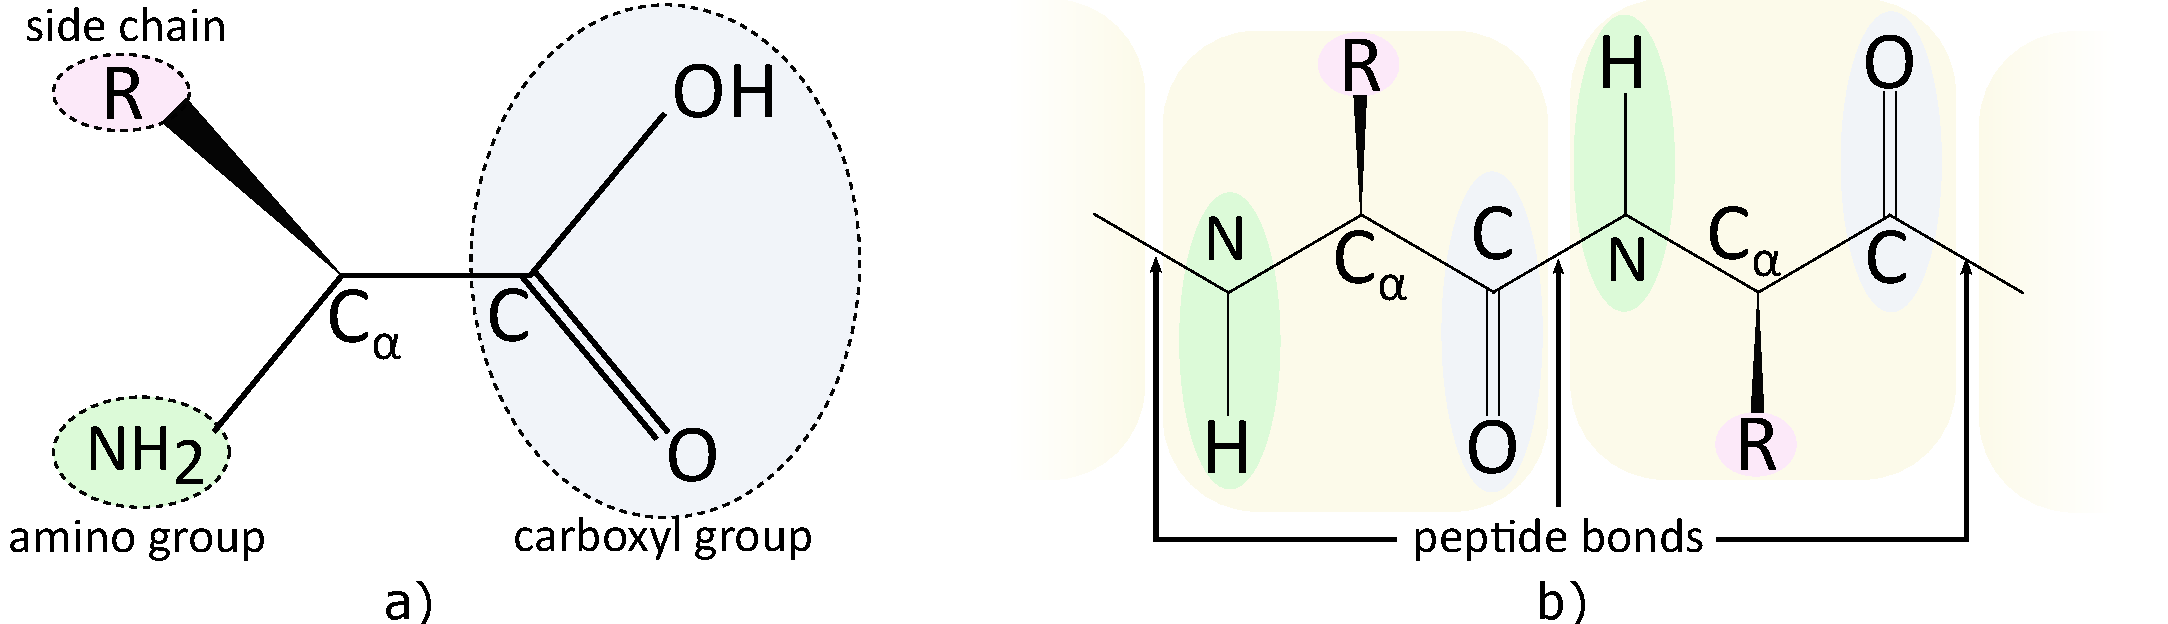
\includegraphics[width=\textwidth]{pictures/aminoacid.pdf} 
  \caption{a) Illustration of a basic amino acid structure. b) Amino acid residues connected into polypeptide chain. It can be noted, that the amino and carboxyl groups are missing atoms, which were released during the formation of peptide bonds as $H_2O$ molecules.}
  \label{Fig:aa}
\end{figure}

During a protein synthesis amino acids are joined together by peptide bonds (covalent bonds), forming polypeptide chains. A peptide bond is formed in a reaction between carboxyl group of one amino acid and amino group of another amino acid (see figure \ref{Fig:aa} b)). As both groups loose atoms that are released as molecule of water during this reaction, the amino acids bonded in polypeptide chains are refereed to as \textit{amino acid residues}. 

Each protein contains at least one long polypeptide chain. This sequence of amino acids, connected by rigid peptide bonds, also known as \textit{backbone}, forms \textit{primary structure} of the protein.

Unlike the peptide bonds, the bonds linking the carboxyl and amino groups to the alpha carbon are free to rotate. Based on these rotations and the patterns of hydrogen bonds that form between hydrogen from amino group and oxygen from corboxyl group, the segments of polypeptide chain can take on various 3D formations. The two most common of those are $\alpha-helices$ and $\beta-sheets$, which are formed by laterally connected $\beta-strands$. These local formations of polypeptide chain are called \textit{secondary protein structures}. Parts of polypeptide chain with absent secondary structures are called \textit{random coils}. See figure \ref{Fig:secondary}.

\begin{figure}[H]
  \centering
  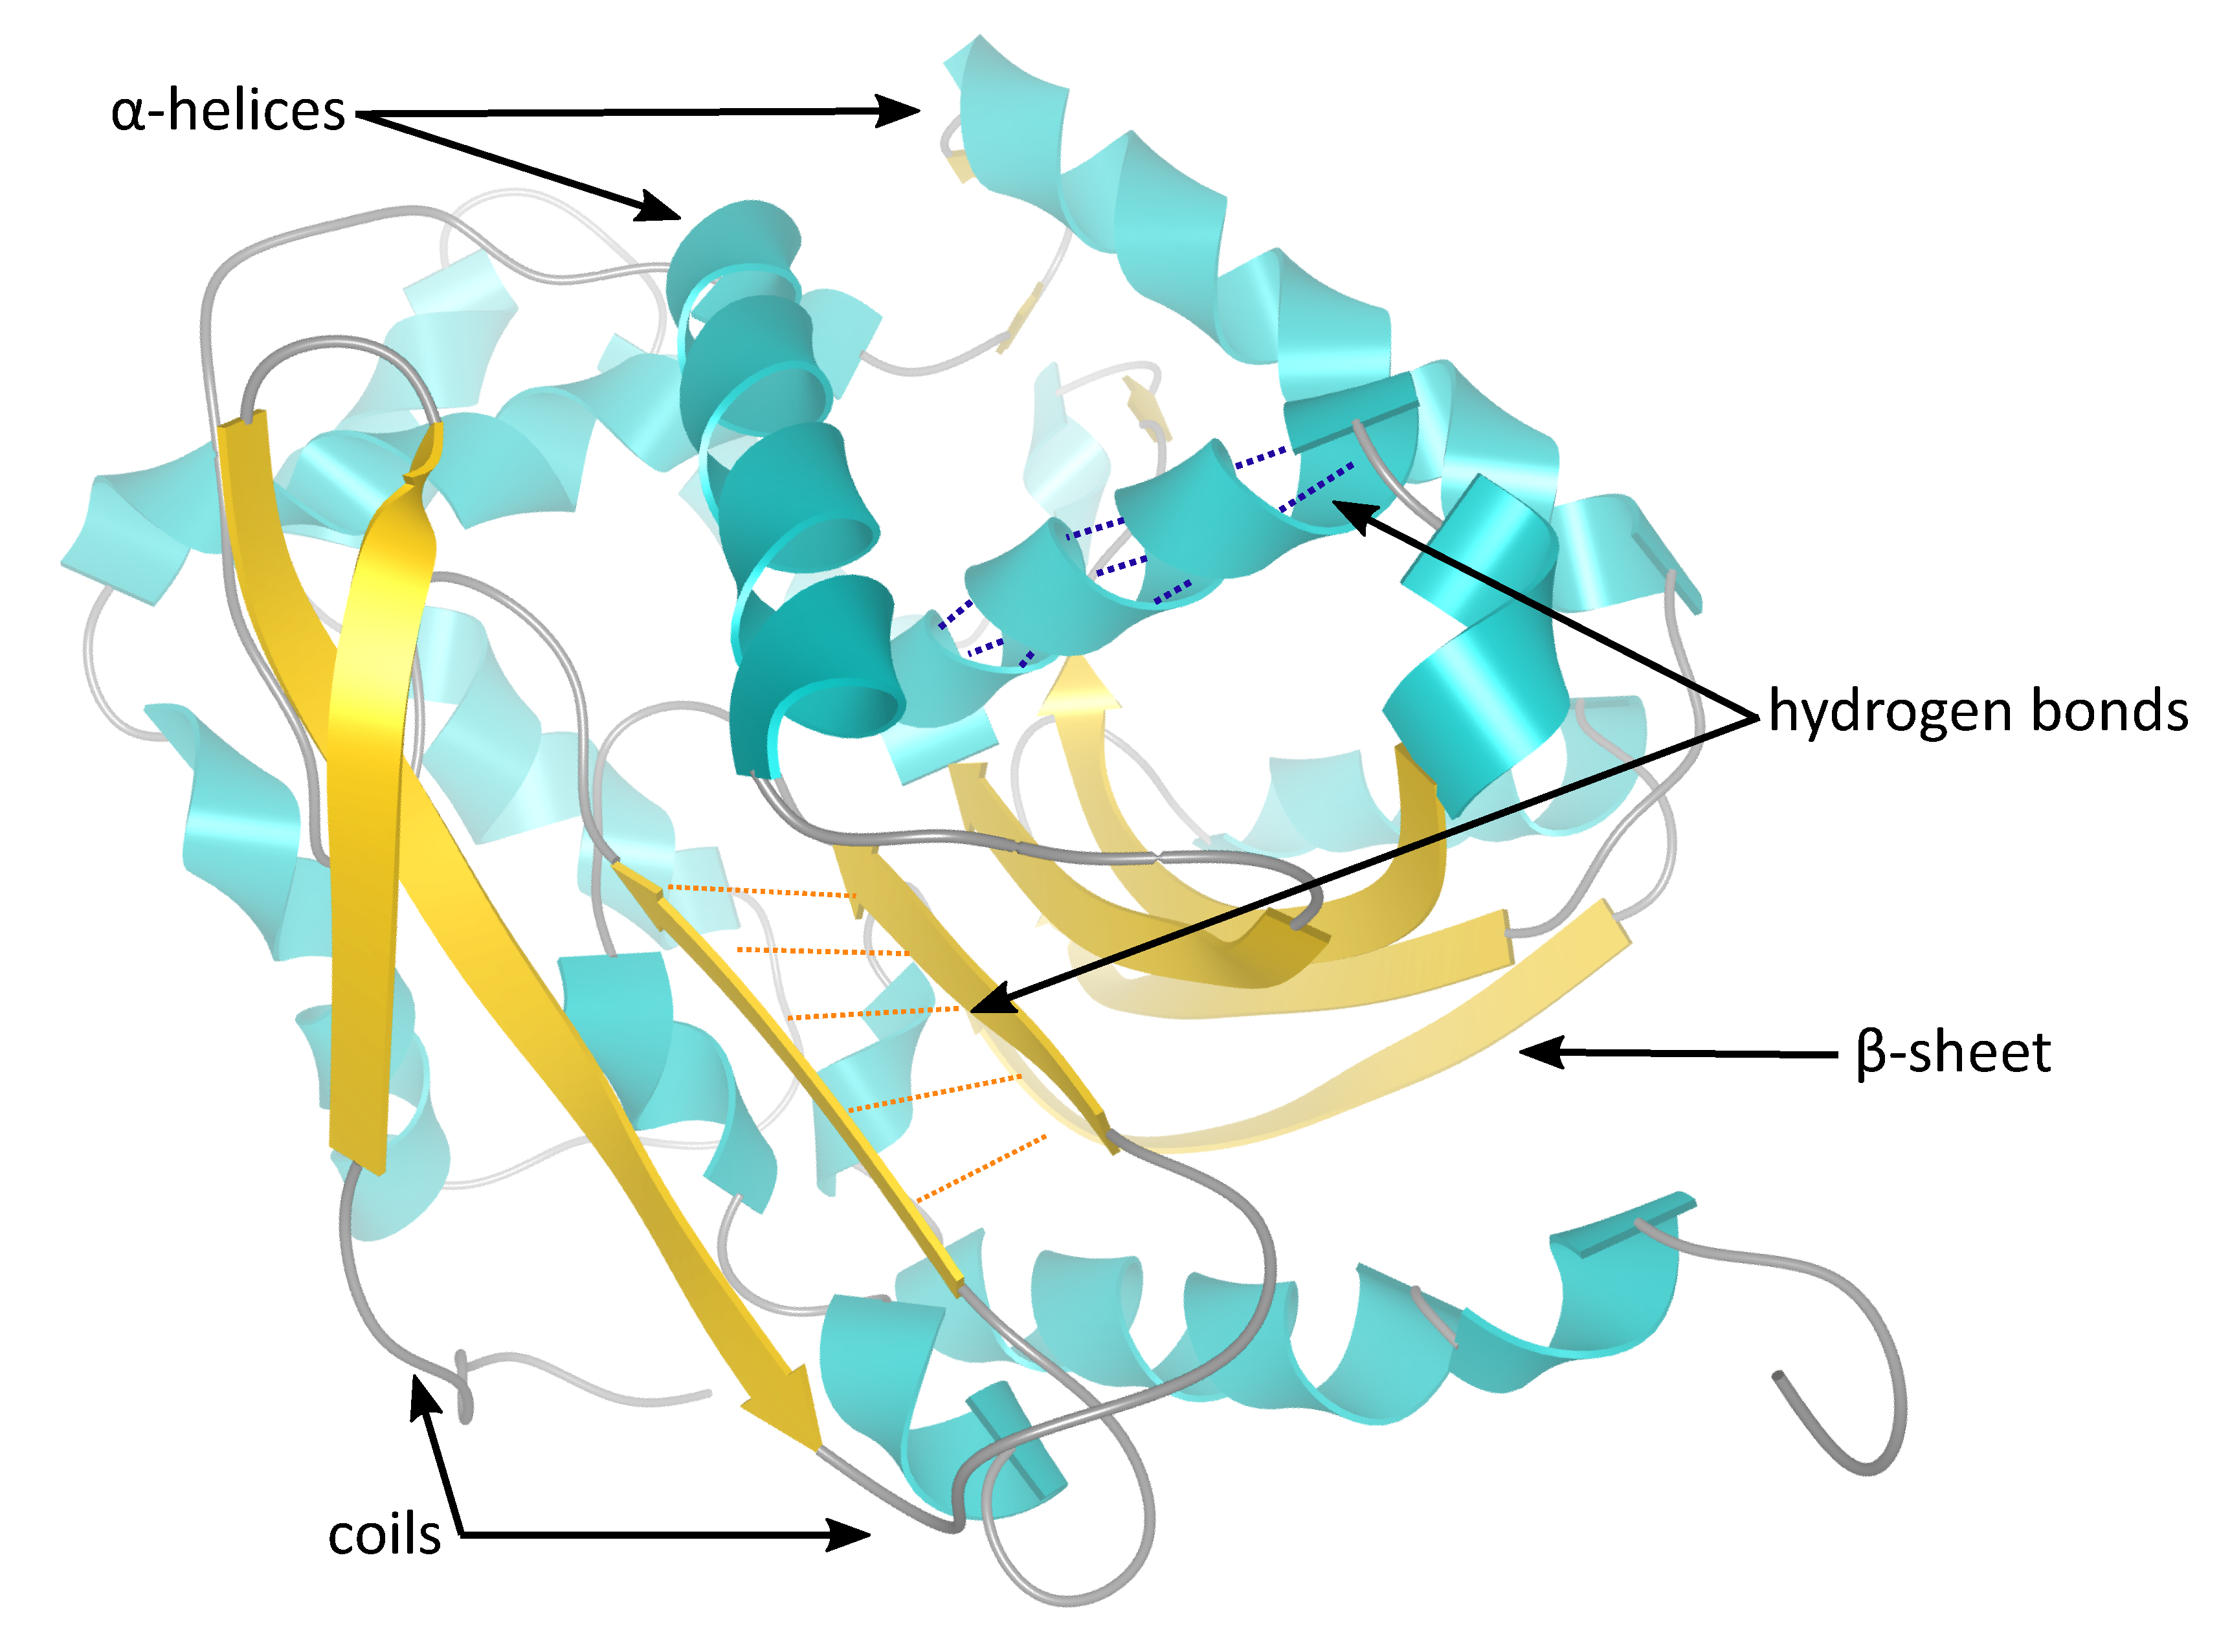
\includegraphics[width=.6\textwidth]{pictures/secondary.pdf} 
  \caption{Typical secondary structures of protein: $\alpha-helices$ (blue), $\beta-strands$ (orange) forming $\beta-sheet$ and \textit{coils}.}
  \label{Fig:secondary}
\end{figure} 

Various side chains of amino acid residues can interact together during the formation of protein. As a result, the secondary structures of the protein are bended and shaped into a  unique 3D structure until the protein attains its minimal energy state. This process is called \textit{protein folding} and it results in a \textit{tertiary protein structure}. The tertiary structure defines the complete spatial arrangement of atoms of one polypeptide chain. Interactions between amino acids of multiple polypeptide chains than define their \textit{quaternary protein structure}.

\subsection{Properties of Proteins}
Previous section described the process of protein attaining its 3D structure. This structure directly influences the way protein is behaving with regards to other molecules and its ability to function properly.

Example of this are the inner voids of the protein. When protein folds, there is naturally some empty space left inside. Depending on the shape of the space we classify four types of inner voids (figure \ref{Fig:voids}): \textit{cavities} -- void space buried deeply inside the protein,  \textit{tunnels} -- connecting cavities with surface of the protein, \textit{channels} -- passing through the whole protein and \textit{pockets} -- shallow dents on the surface of the protein.

\begin{figure}[H]
  \centering
  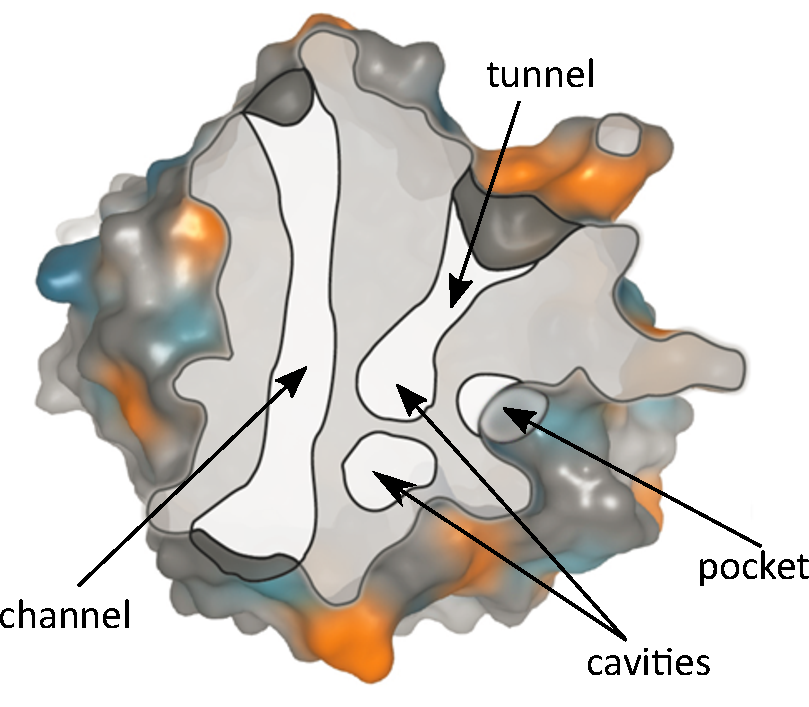
\includegraphics[width=.5\textwidth]{pictures/Voids.pdf} 
  \caption{Types of inner voids of protein. Image adapted from \cite{Strnad2014Thesis}}
  \label{Fig:voids}
\end{figure}

These inner voids can significantly influence the reactivity of the protein since they contain \textit{active site}. Active site is a region of reactive amino acids, where other smaller molecules can bind to protein and undergo a chemical reaction that changes their properties. This place is often buried deep inside the protein and its accessibility is thus limited by the size, shape and physico-chemical properties of the tunnels leading to it. However, the binding site can be located also in shallower pockets on protein surface. In several types of proteins, these binding sites serve for interacting with other proteins.

On the other hand, proteins containing channels (also called pores) occupy entirely different function. They are often found in the membranes of the cells, where the geometry and properties of the channels are responsible for regulating the molecules that can pass through the cell membrane. They are often specific to one type of molecule -- e.g. water, and no other molecules can pass through them in or out of the cell.

As noted above, the reactivity and functions of the proteins are given by their geometry as well as by their physico-chemical properties. These properties are analogous to the properties of the their amino acids:

\begin{itemize}
\setlength\itemsep{0.5pt}
\item{\textit{Polarity and Partial Charge}} \\ 
In a molecule of water, hydrogen atoms are bound to highly electronegative oxygen atom. The electronegativity of oxygen causes higher concentration of electrons on its side of hydrogen bonds and thus a separation of positive and negative electric charge (electric dipole). This phenomenon occurs also in several so called \textit{polar} amino acids. The amount of separated charge is usually lower than fundamental charge, therefore it is called \textit{partial charge}. 
\item{\textit{Donor / Acceptor}} \\
Amino acids participating in hydrogen bonds can be classified as \textit{hydrogen donors} or \textit{hydrogen bond donors} if they contain the hydrogen atoms participating in this bonds. Amino acids on the other side of the bond are called \textit{hydrogen acceptors}. Note that amino acids participating in multiple hydrogen bonds can be donors and acceptors at the same time.
\item{\textit{Hydrophobicity}} \\
 Amino acids are called \textit{hydrophobic} if they seemingly repel water. Unlike \textit{hydrophilic} amino acids, they are not polar and thus cannot create bonds with polar molecules of water.
\end{itemize}

Most of the proteins contain hydrophobic amino acids at their core, while their surface is covered by polar amino acids. They are in contact with outer environment -- \textit{solvent}, where they can form hydrogen bonds.

So far, when discussing the properties of proteins, we have assumed the static 3D structure. However, due to constant physical forces taking place between millions of atoms of proteins and surrounding solvents, the structure of the protein is not static and when studying the proteins one has to consider so called \textit{molecular dynamics (MD)}. This term generally denotes the simulation or the captured interval of atom movement that constantly changes not only the shape but consequently also properties of observed proteins. 

\section{Problem Formulation}
Now that the reader is familiar with basic biochemical terminology, we can formulate the specific problems that will be the focus of this thesis. It was already hinted that proteins can participate in various kinds of intermolecular interactions. In this thesis we will focus on two typical types of interactions: a) protein-ligand interactions and b) protein-protein interactions.

\subsection{Protein-Ligand Interactions} 
In biochemical terminology ligand denotes a small molecule that binds to a protein, where the consequential reaction changes both, the target protein as well as the ligand itself. Analysis of protein-ligand docking (the act of ligand travelling through the protein tunnel and binding to the active site) has application in different fields of biochemistry such as protein engineering or drug design. The typical goal of protein engineering research is changing of protein properties by mutating some of its amino acids to make it, e.g. more stable under high temperature conditions or more reactive with a particular type of ligand. In drug design the goal is to find or adjust protein-ligand combinations, such that their mutual reaction would synthesize new drug from the ligand.
However, in both cases the researchers are looking for the answers to the following questions:
\begin{itemize}
\setlength\itemsep{0.5pt}
\item{Can the ligand pass through the tunnel leading to the active site?}
\item{If not, which parts of the tunnels are causing problems?}
\item{Is it the geometrical bottleneck, that prevents the ligand from passing through the tunnel?}
\item{Are the physico-chemical properties of the tunnel amino acids responsible for repelling the ligand from the active site?}
\item{Can these problems can be resolved by mutating the protein amino acids?}
\end{itemize}

There is already great amount of published work aiming to answer these questions either by studying the tunnel properties or by directly simulating the transportation of the ligand to the active site. However, with the complexity of protein structures in combination with the ever-changing molecular dynamics, the answers are not trivial. Figure \ref{Fig:trajectory} for example depicts trajectory of a ligand in a MD simulation consisting of 50 000 time steps. It is apparent, that further analysis is necessary to identify significant parts and patterns in this simulation. 

\begin{figure}[H]
  \centering
  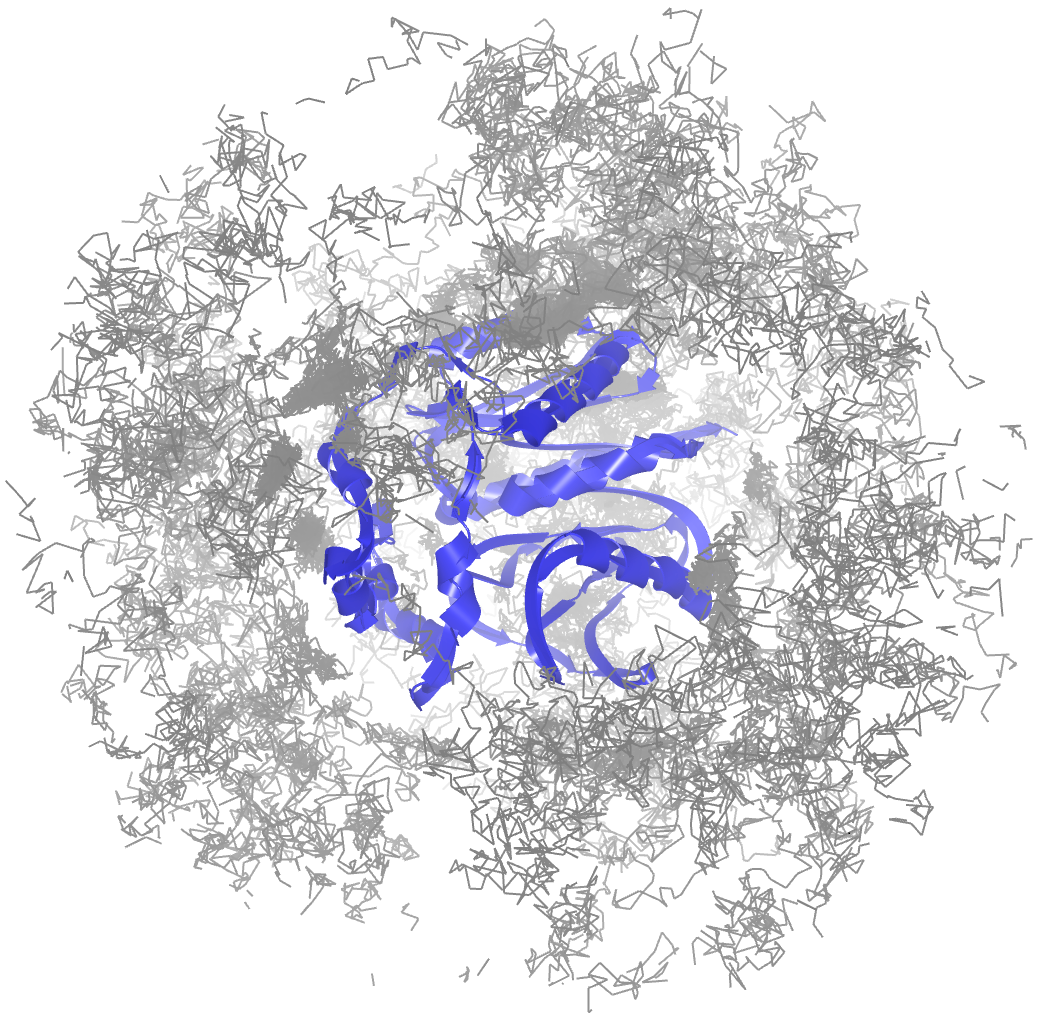
\includegraphics[width=0.5\linewidth]{pictures/lig_movement.png} 
  \caption{Ligand trajectory (gray) in a simulation containing 50 000 time steps. The protein chain is depicted in blue.}
  \label{Fig:trajectory}  
\end{figure} 

\subsection{Protein-Protein Interactions}
Most of the proteins responsible for various functions in cellular life are operating in larger multi-protein complexes. For example a family of SMC complexes (structural maintenance of chromosomes) govern the organisation of DNA in the cell nucleus. However, in order to interpret their functions properly, it is vital to understand the way the protein are interacting together in these complexes. Mapping the \textit{contact zones} consisting of surface amino acids interacting between the proteins is time consuming process that requires expensive laboratory experiments. Several computational tools therefore aim to reduce the amount of necessary experiments by predicting the possible docking conformations of given proteins. These tools can produce tens to hundreds of possible solutions and it is than up to biochemists to identify the plausible ones. To determine this, the researchers are trying to answer following questions:

\begin{itemize}
\setlength\itemsep{0.5pt}
\item{Which pairs of interacting amino acids are present in a given configuration?}
\item{Which configurations contain a specific interacting pair of
amino acids?}
\item{How close are the amino acids in the contact zone and which
are the closest ones?}
\item{How similar and different are the contact zones in different configurations?}
\item{What are the physico-chemical properties of the amino acids
in the contact zone?}
\end{itemize}

The identification of relevant docking conformations is currently not well supported and the domain experts performing this task by visually comparing the 3D representations of the docked proteins (see figure \ref{Fig:problem}). This approach suffers from high visual complexity, occlusion and imprecise identification of contact pairs of amino acids. It is therefore very difficult to answer the posed questions.

\begin{figure}[H]
  \centering
  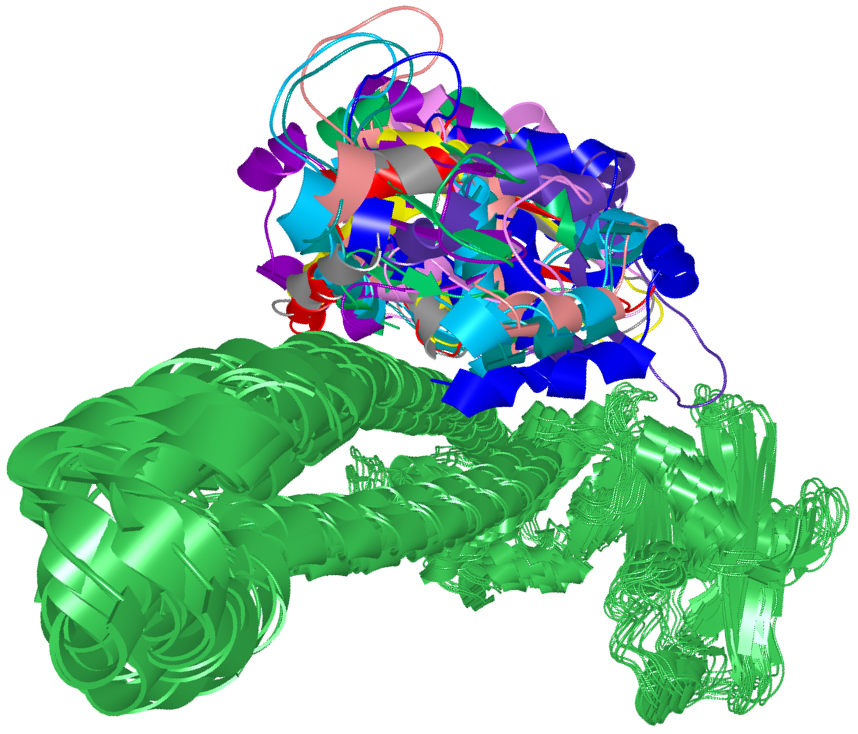
\includegraphics[width=0.5\linewidth]{pictures/problem.png} 
  \caption{Superposition of several possible conformations between two proteins. The set of green protein instances corresponds to one of the proteins in the interaction, the colored components represent the second protein in different conformations.}
  \label{Fig:problem}  
\end{figure} 

\subsection{Summary}
In-silico simulations of chemical processes such as molecular docking reduce the time and costs necessary for in-vitro experiments. Yet, the complexity of the generated data almost always calls for further analysis. It is usually up to domain expert to judge the soundness of data and derive conclusions. Without popper tools, this can be difficult and tedious assignment. However, visualization metaphors supporting particular research tasks and  their combinations in an interactive visual analytics's system can significantly speed up the analysis procedure and help with relieving interesting patterns and relationships in data. 

In this work we will present the current state of the art techniques in the visualization and visual analysis of intermolecular interactions of proteins and analyse, how they address the questions posed in the previous sections. We will identify the unsolved problems occurring in the literature, then present the proposed solutions and results that have already been achieved. We will also outline the possibilities for further research.